\section*{Figures}

\listoffigures

\clearpage

\begin{figure}%[tbhp]
\centering
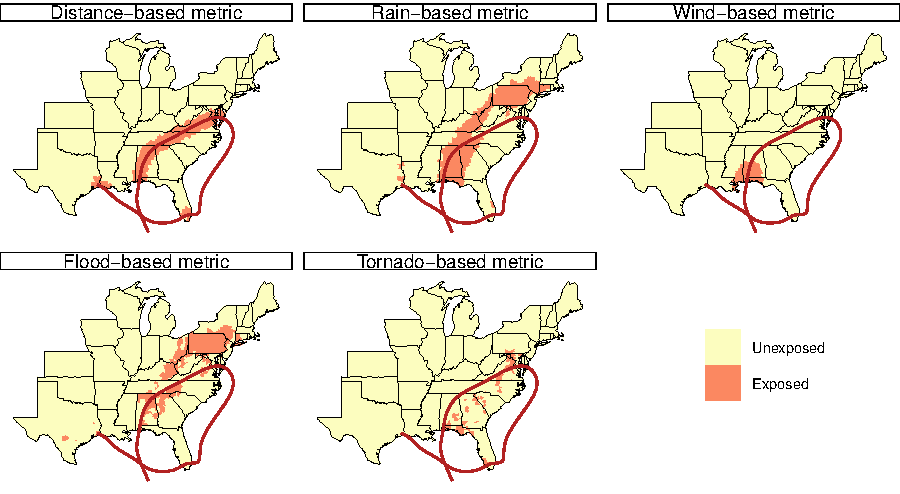
\includegraphics[width=16cm]{ivanonly.pdf}
\caption{Counties classified as exposed to Hurricane Ivan (2004) under each
exposure metric (Table~1). The red line shows the track of Hurricane Ivan 
based on the revised Atlantic hurricane database \ac{HURDAT2}~\citep{landsea2013}.
Similar maps for other large-extent storms are given in Figure~S3.}
\label{fig:ivanexposure} 
\end{figure}

\clearpage

\begin{figure}%[tbhp] 
\centering 
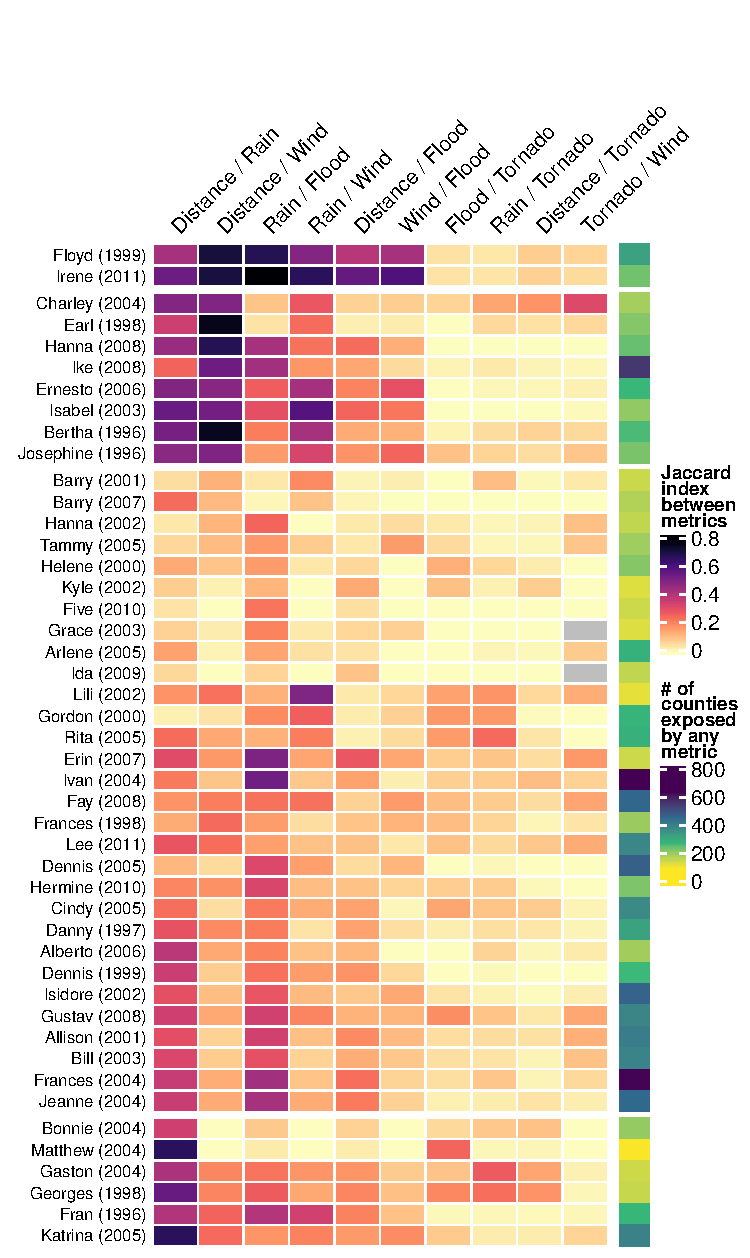
\includegraphics[width = 0.6\linewidth]{jaccard_heatmap.pdf} 
\caption{Heatmap of Jaccard index values for specific exposure metric pairs
within storms. Only storms between~1996 and~2011, and for which at least~250
counties were exposed based on at least one metric, are included. The color of
each cell within the main heatmap indicates the value of the Jaccard index
(proportion of counties classified as exposed by both metrics out of storms
classified as exposed by either metric) for a given pair of metrics for a given
storm. Storms are displayed within clusters that have similar patterns in
county-level exposure agreement for metric pairs, based on hierarchical
clustering using the complete link method~\citep{murtagh2012algorithms} (i.e.,
storms in the same cluster tend to have similar patterns for the pairwise
strength of agreement among metrics); columns are also ordered based on
hierarchical clustering. The colors to the right of the main heatmap for each
storm indicate the total number of counties classified as exposed to the storm
by any of the five metrics, providing an estimate of storm extent. Maps are
available showing the counties identified as exposed under each of five metrics
for the widest-extent storm in each cluster: Hurricane Ivan (2004)
(Figure~\ref{fig:ivanexposure}) and Hurricanes Floyd (1999), Lee (2011), Cindy
(2005), and Katrina (2005) (Figure~S3).} 
\label{fig:jaccard}
\end{figure}

\clearpage

\begin{figure}%[tbhp] 
\centering
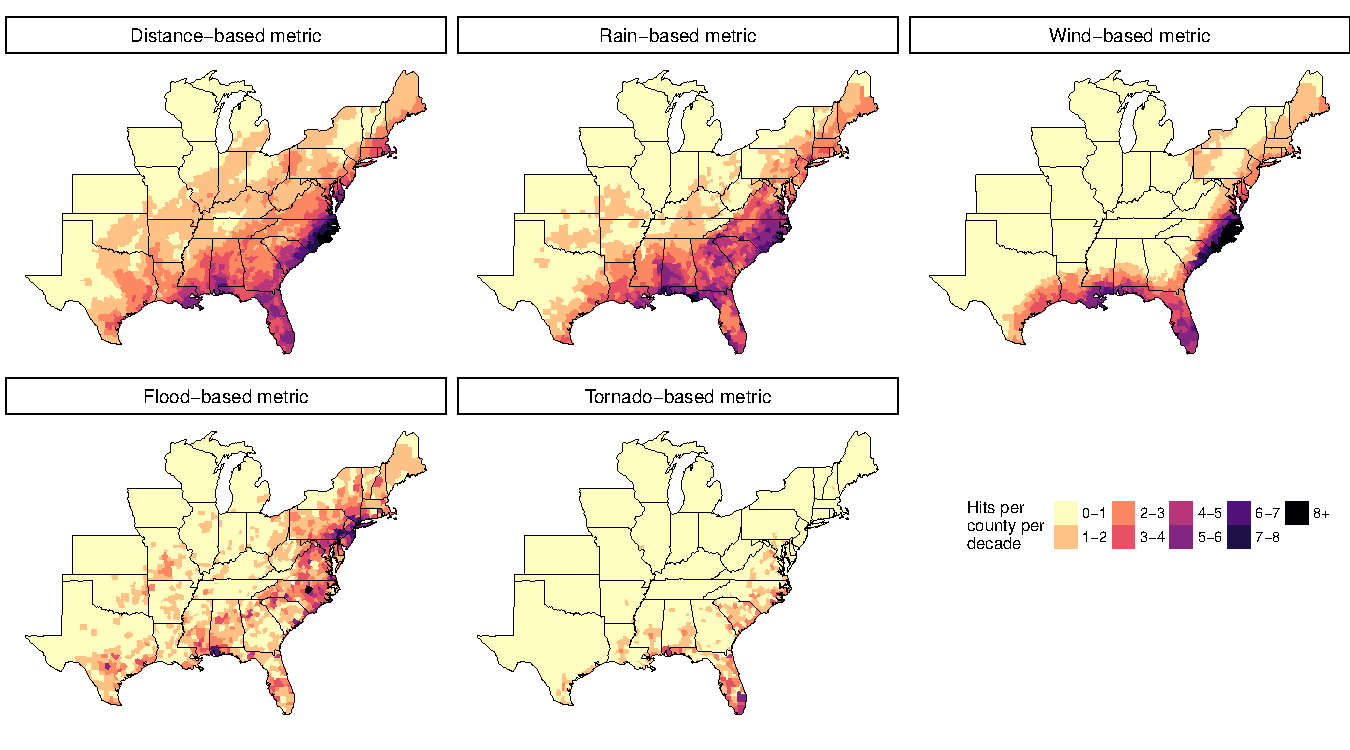
\includegraphics[width=15cm]{averageexposureonly.pdf} 
\caption{Average number of storm exposures per decade in U.S. counties for each
exposure metric. The criteria behind each of the five metrics is given in Table
\ref{tab:exposuremetrics}. The years used to estimate these averages are based
on years of available exposure data (distance and wind:~1988\,--\,2015; rain:
1988\,--\,2011; flood and tornado:~1996\,--\,2015). Similar patterns persist when
analysis is restricted to years with all exposure data available (1996\,--\,2011;
Figure~S5).} 
\label{fig:averageexposure} 
\end{figure}

\clearpage

\begin{figure*}%[tbhp]
\centering
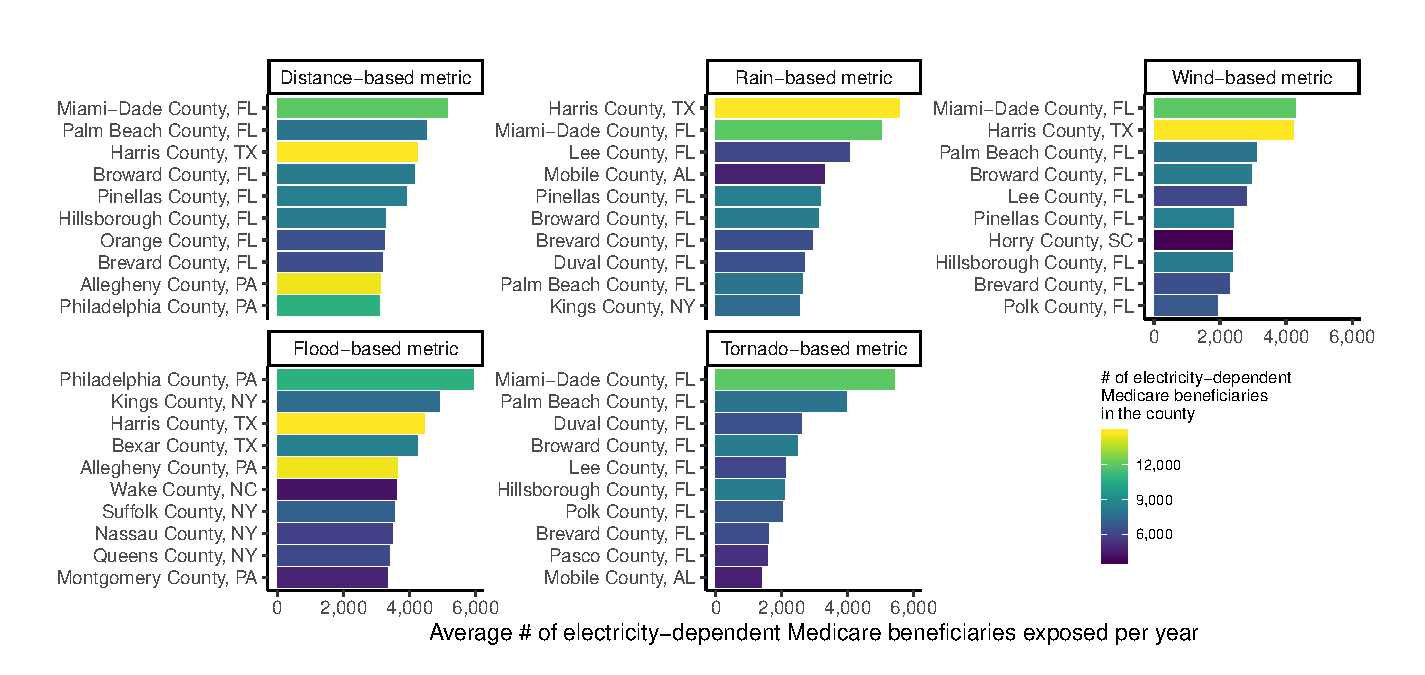
\includegraphics[width=15.5cm]{topelecdependexposure}
\caption{Counties with the highest estimated physical exposure among
electricity-dependent Medicare beneficiaries exposed to storms per year in U.S.
counties for each exposure metric. The criteria behind each of the five metrics
are given in Table~1 [use ref] and details of the physical exposure
calculation are given in the Methods. The color of each bar indicates the
number of Medicare beneficiaries in the county reliant on electricity-dependent
medical and assistive equipment as of July~2017~\citep{empower}. The length of
each bar shows the average expected number of these electricity-dependent
Medicare beneficiaries exposed to tropical storms per year based on a given
exposure metric.}
\label{fig:topelecdependexposure}
\end{figure*}

\clearpage

\begin{figure}[tbhp!]
\centering
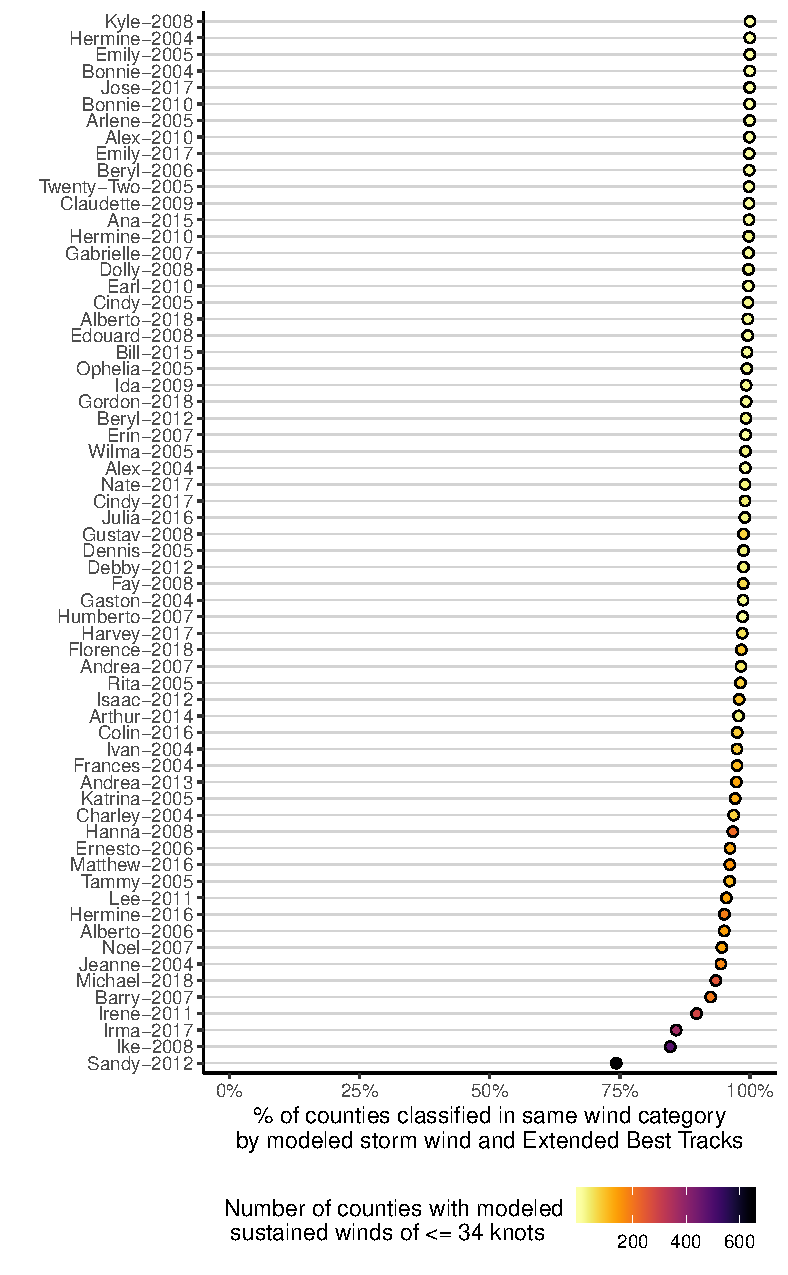
\includegraphics[width=0.6\linewidth]{windcomparison}
\caption{Comparison of estimated wind categories from modeled sustained wind
speed (as used for the wind exposure metric in the main
text;~\citep{stormwindmodel}) versus sustained wind speed determined from the
revised Atlantic hurricane database \ac{HURDAT2}~\citep{landsea2013}. In
\ac{HURDAT2}, wind radii were available for study storms from~2004\,--\,2015
and gives estimates of the maximum radii to which storm winds of 34~\si{\knot},
50~\si{\knot}, and 64~\si{\knot} extended in each four quadrant of the storm at
each of the 6-\si{\hour} storm track observations. We interpolated this data
to~15-\si{\minute} increments and assessed a county as exposed to winds at or above
one of these cutoffs if its population mean center was within~85\% of the
maximum radius for that wind speed in its quadrant of the storm. For each
county in each of the available storms, we also calculated the modeled wind
speed~\citep{stormwindmodel} and then categorized this value into the same
categories available for the \ac{HURDAT2} wind radii ($<$34~\si{\knot};
34\,--\,49.9~\si{\knot}; 50\,--\,63.9~\si{\knot}; $\ge$64~\si{\knot}). Each
point in this graph shows, for a storm, the percent of counties in which the
wind category ($<$34~\si{\knot}; 34\,--\,49.9~\si{\knot};
50\,--\,63.9~\si{\knot}; $\ge$64~\si{\knot}) was the same based on both modeled
winds and the \ac{HURDAT2} wind radii. Only storms with at least one county
with sustained wind of~$\ge$34 \si{\knot}, based on the \ac{HURDAT2} wind
radii, are shown. Hurricanes Sandy (2012) and Ike (2008) were he two storms
with the worst agreement between these two sets of wind data; maps with further
comparisons between the two data sources for these two storms are given in
Figure~\ref{fig:windexamples}.}
\label{fig:windcomparison}
\end{figure}

\begin{figure}[tbhp!] \centering
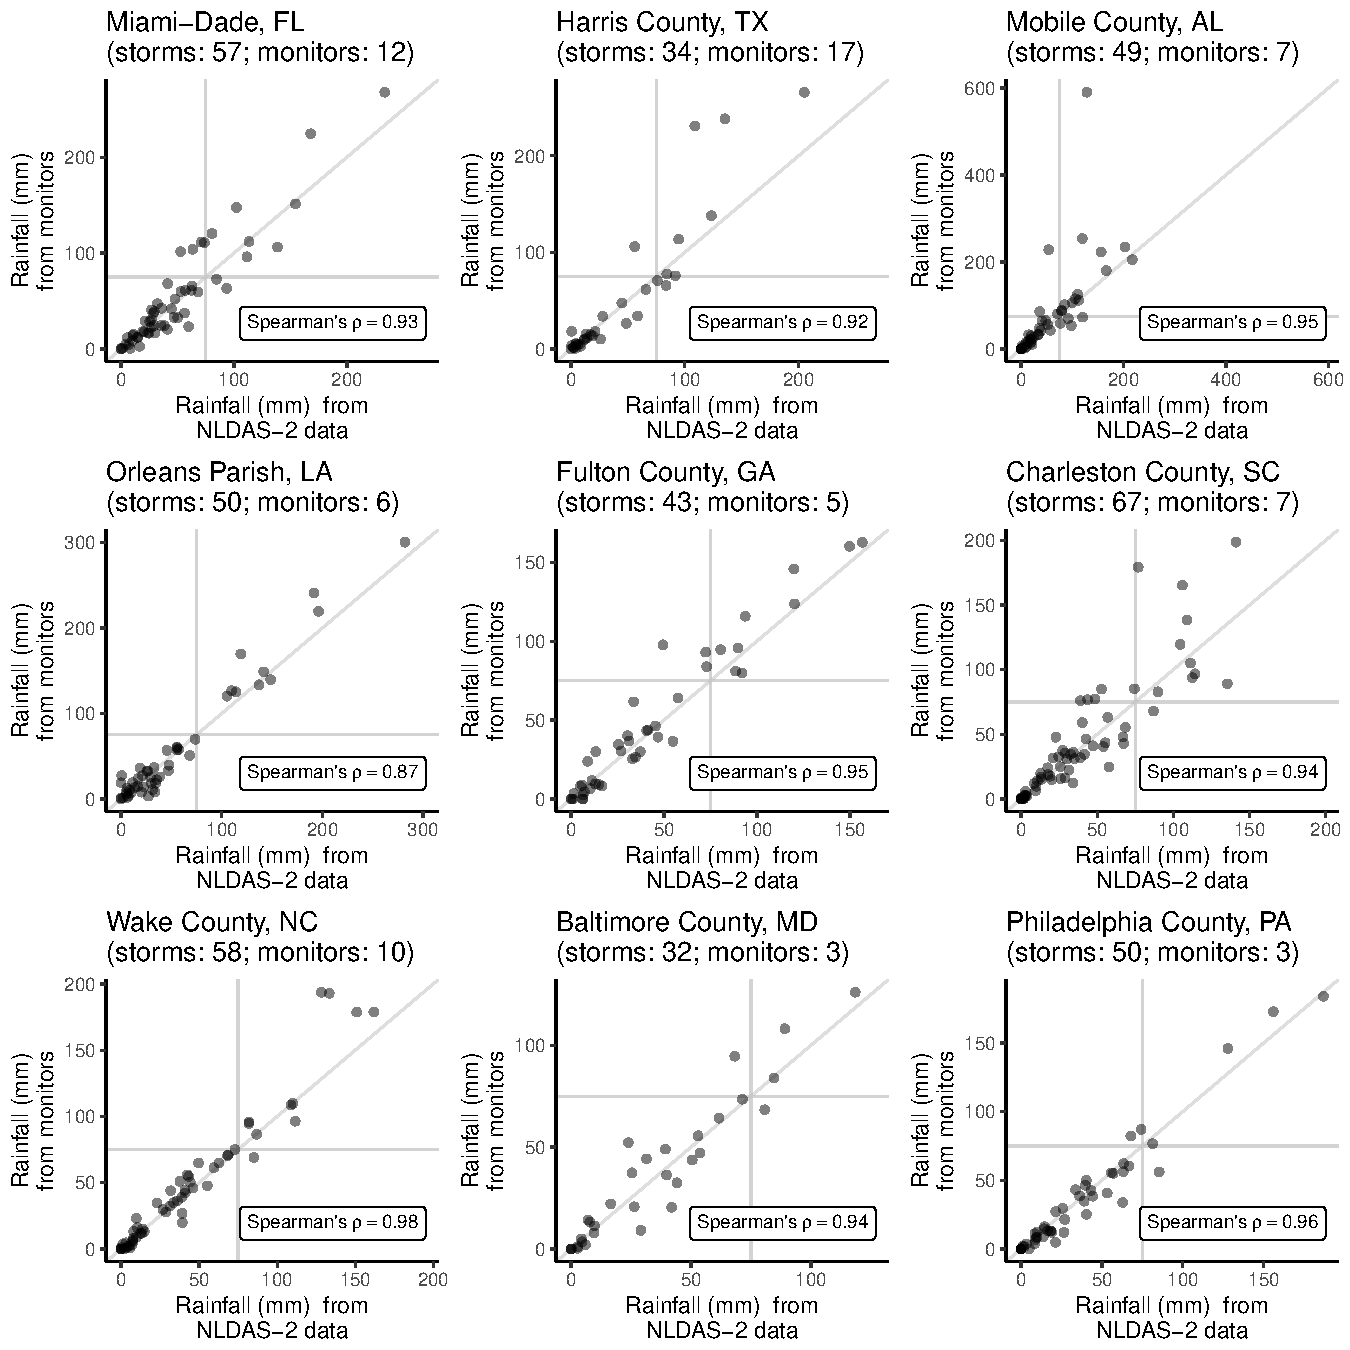
\includegraphics[width=0.9\linewidth]{raincomparison} \caption{Comparison of
county-level rain exposure based on the reanalysis data used for exposure
assessment in this study \ac{NLDAS-2}~\citep{rui2013nldas,
alhamdan2014environmental} and ground-based weather
stations~\citep{menne2012overview, rnoaa, countyweather}. Each small graph
shows a sample county, and each point on the graph represents a tropical storm
that came within~500 \si{\kilo\metre} of the population mean center of the county.
The x-axis shows the estimated cumulative rainfall (in millimeters) from two
days before to one day after the storm's closest approach to the county based
on the county-aggregated \ac{NLDAS-2} recipitation data used to measure rain
exposure in our main analysis. The ground-based observations (y-axis) are based
on collecting precipitation data from available weather stations in the county,
1988\,--\,2011, summed over the same period from two days before to one day
after the storm's closest approach for each available station. These cumulative
station-based precipitation totals were then averaged across all available
stations in the county to create a county-wide estimate of cumulative
storm-related precipitation for each storm in the county. Horizontal and
vertical lines show the threshold used to classify a storm as exposed based on
cumulative rainfall; storms in the lower left and upper right quadrants are
classified the same regardless of whether reanalysis or station-based
precipitation data is considered, while storms in the upper left and lower
right quadrants would be classified differently. The number of storms within
each county and the average number of stations reporting rainfall during the
county's storms are given above each plot. Note that x- and y-axis ranges
differ by county. An estimate of the rank correlation
(Spearman's~$\rho$~\citep{spearman1904proof}) between measurements from the two
rain data sources is also shown on each graph.} \label{fig:raincomparison}
\end{figure}

\begin{figure}[tbhp!]
\centering
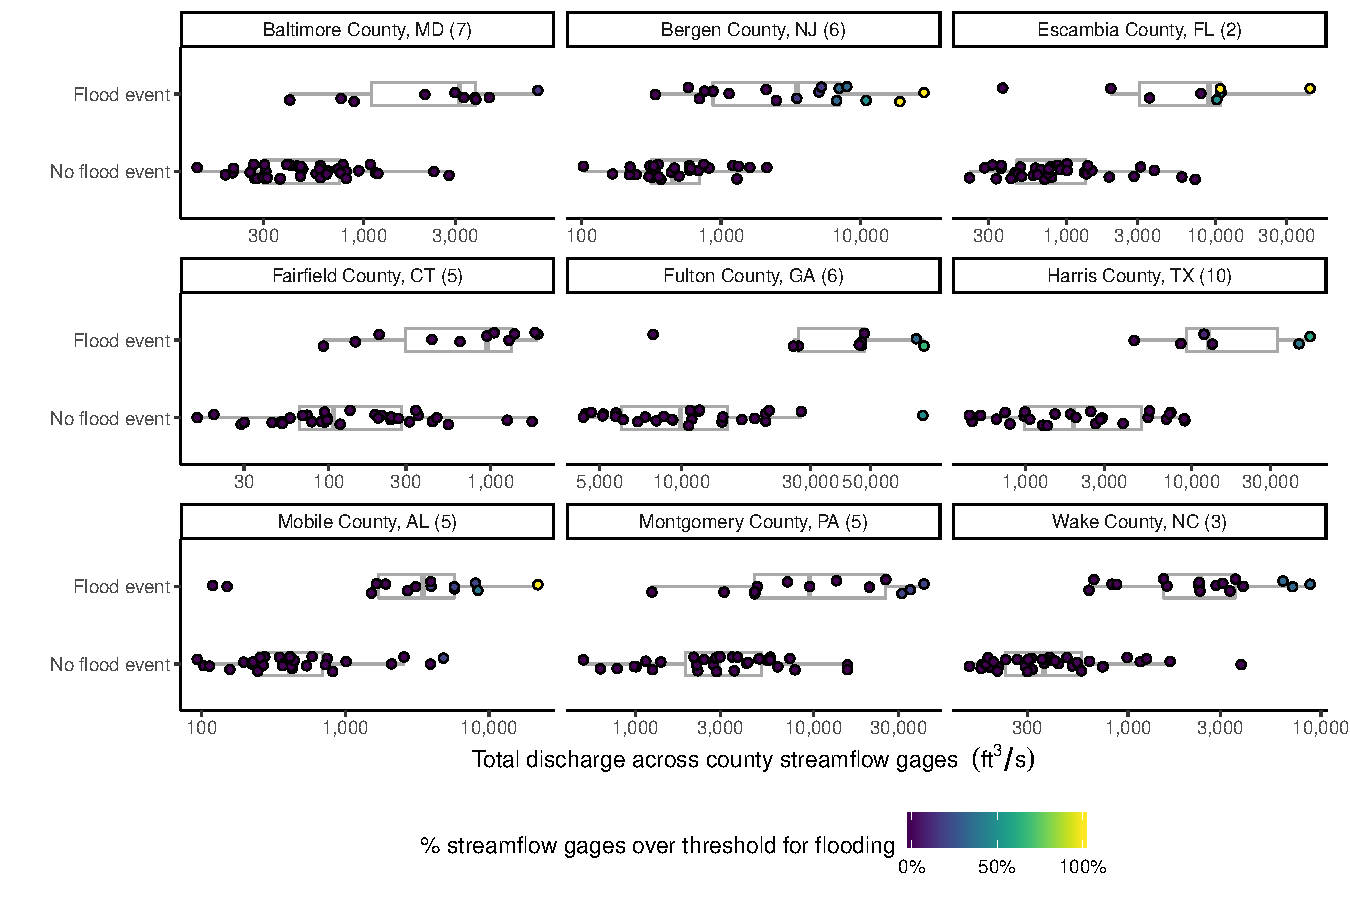
\includegraphics[width=0.8\linewidth]{floodcomparison}
\caption{Comparison of for a sample of study counties of flood status, based on
NOAA Storm Events listings~\citep{stormevents, noaastormevents}, with total
streamflows at county streamflow gages during tropical storms~\citep{usgsgages,
countyfloods, dataRetrieval}. Each panel represents a separate county. For each
county, we first identified all streamflow gages in the county that had
complete data for Jan.~1~1996\,--\,Dec.~31,~2015. The number of streamflow
gages meeting this criterion are given in parentheses beside the county's name
in the panel title. This analysis covered tropical storm that came
within~500~\si{\kilo\metre} of each sample county between~1996 and~2015. In the
graphs, each point represents a single tropical storm, and the point's position
along the x-axis shows the highest daily total streamflow (cubic feet /
second), summed across all identified streamgages in the county, for a five-day
window centered on the day of the storm's closest approach to the county. The
y-axis separates storms for which a flood event was reported in NOAA's Storm
Events database for the county with a start date within the five-day window of
the storm's closest approach to the county~\citep{stormevents,
noaastormevents}. Boxplots are added to show the distribution of the total
streamflow measurements across storms in the county for storms grouped by
whether or not they were linked with a flood event based on the NOAA Storm
Events data. The color of each point gives the percent of streamflow gages in
the county with a daily streamflow that exceeded a threshold of flooding (the
streamgage's median value for annual peak flow~\citep{countyfloods}) on any day
during the five-day window.  Note that the x-axis scales differ by county,
depending on the number of streamflow gages and typical flow rates for each
gage, and are on a log-10 scale.}
\label{fig:floodcomparison}
\end{figure}


